
%%%%%%%%%%%%%%%%%%%%%%% file typeinst.tex %%%%%%%%%%%%%%%%%%%%%%%%%%%%%%
%
% This is the LaTeX source for the instructions to authors using
% the LaTeX document class SVMultln with class option 'lnicst'
% for contributions to the Lecture Notes of the Institute for
% Computer Sciences, Social-Informatics and
% Telecommunications Engineering series.
% www.springer.com/series/XXXX       Springer Heidelberg 2007/08/05
%
% It may be used as a template for your own input - copy it
% to a new file with a new name and use it as the basis for
% your article. It contains a few tweaked sections to demonstrate
% features of the package, though.
%
% If you have not much experiences with Springer LaTeX support,
% you should better use the special demonstration file "lnicst.tex"
% included in the LaTeX package for LNICST as template.
%
%%%%%%%%%%%%%%%%%%%%%%%%%%%%%%%%%%%%%%%%%%%%%%%%%%%%%%%%%%%%%%%%%%%%%%%%

%\documentclass{sig-alternate-10pt}
\documentclass{sig-alt-hotnets}
\usepackage{amssymb}
\setcounter{tocdepth}{3}
%\usepackage{hyperref}
\usepackage[english]{babel}
%\usepackage[pdftex]{graphicx}
\usepackage[nolist]{acronym}
\usepackage{subfigure}
\usepackage[normalem]{ulem}
\usepackage{url}
\urldef{\mailsa}\path|mukerjee@cs.cmu.edu|
\usepackage[pdfpagelabels,hypertexnames=false,breaklinks=true,bookmarksopen=true,bookmarksopenlevel=2]{hyperref}
%\renewcommand{\labelitemi}{$\bullet$}
\usepackage{cite}

%%%
%%% MISC
%%%t
\usepackage{ifthen}
\usepackage{color}
\usepackage{booktabs}  % for toprule and midrule in tables

%%%
%%% COMMENTS / TODOS
%%%
\newcommand{\showComments}{yes}

\newcommand{\note}[2]{
    \ifthenelse{\equal{\showComments}{yes}}{\textcolor{#1}{#2}}{}
}
\newcommand{\TODO}[1]{%
	\addcontentsline{tdo}{todo}{\protect{#1}}%
	\note{red}{TODO: #1}
}
\newcommand{\srini}[1]{\note{magenta}{Srini: #1}}
\newcommand{\dongsu}[1]{\note{red}{Dongsu: #1}}
\newcommand{\fahad}[1]{\note{red}{Fahad: #1}}
\newcommand{\jwb}[1]{\note{cyan}{jwb: #1}}
\newcommand{\michel}[1]{\note{blue}{Michel: #1}}
\newcommand{\aditya}[1]{\note{violet}{Aditya: #1}}
\newcommand{\ashok}[1]{\note{blue}{Ashok: #1}}
\newcommand{\dga}[1]{\note{green}{dga: #1}}
\newcommand{\hyeontaek}[1]{\note{red}{Hyeontaek: #1}}
\newcommand{\prs}[1]{\note{purple}{Peter: #1}}
\newcommand{\boyan}[1]{\note{red}{Boyan: #1}}
\newcommand{\david}[1]{\note{green}{David: #1}}
\newcommand{\matt}[1]{\note{blue}{Matt: #1}}


\makeatletter \newcommand{\listoftodos}
{\section*{Todo List} \@starttoc{tdo}}
\newcommand{\l@todo}
{\@dottedtocline{1}{0em}{2.3em}} \makeatother

\newcommand{\comment}[1]{}


%%
%% TIKZ to represent graphs and diagrams
%%

\usepackage{tikz}
\usepackage{tkz-graph}
\usetikzlibrary{shapes,arrows}

\newcommand{\entrynode}[1]{
  \SetVertexNormal[Shape      = circle,
                   FillColor  = black,
                   LineWidth  = 0pt,
                   MinSize    = 0pt]
  \Vertex[L={\tiny\,}]{#1}
  \SetVertexNormal[Shape      = circle,
                   FillColor  = white,
                   LineWidth  = 2pt]
}

\SetUpEdge[lw         = 1.5pt,
           color      = black,
           labelcolor = white,
           labeltext  = red,
           labelstyle = {sloped,draw,text=blue}]

\tikzset{node distance = 2cm}


%%%
%%% DOCUMENT
%%%

\begin{document}

%\mainmatter  % start of an individual contribution

% first the title is needed
\title{Packet Processing on the GPU}

% the name(s) of the author(s) follow(s) next
%
% NB: Chinese authors should write their first names(s) in front of
% their surnames. This ensures that the names appear correctly in
% the running heads and the author index.
%
\numberofauthors{3}
\author{
\alignauthor
Matthew Mukerjee\\
	\affaddr{Carnegie Mellon University}\\
	\email{mukerjee@cs.cmu.edu}
\alignauthor
David Naylor\\
	\affaddr{Carnegie Mellon University}\\
	\email{dnaylor@cs.cmu.edu}
	\alignauthor
Bruno Vavala\\
	\affaddr{Carnegie Mellon University}\\
	\email{bvavala@cs.cmu.edu}
} 

\maketitle


\vspace{-10pt}

\begin{abstract}

Packet processing in routers is traditionally implemented in hardware;
specialized ASICs are employed to forward packets at line rates of up to 100
Gbps. Recently, however, improving hardware and an interest in complex packet
processing has prompted the networking community to explore software routers;
though they are more flexible and easier to program, achieving forwarding rates
comparable to hardware routers is challenging.

Given the highly parallel nature of packet processing, a GPU-based router
architecture is an inviting option (and one which the community has begun to
explore). In this project, we explore the pitfalls and payoffs of implementing
a GPU-based software router. 

\end{abstract}

\section{Introduction}

There are two approaches to implementing packet processing functionality in
routers: bake the processing logic into hardware, or write it in software. The
advantage of the former is speed; today's fastest routers perform forwarding
lookups in dedicated ASICs and achieve line rates of up to 100 Gbps (the
current standard line rate for a core router is 40 Gbps)\cite{Han}. On the
other hand, the appeal of software routers is programability; software routers
can more easily support complicated packet processing functions and can be
reprogrammed with updated functionality.

Traditionally, router manufacturers have opted for hardware designs since
software routers could not come close to achieving the same forwarding rates.
Recently, however, software routers have begun gaining attention in the
networking community for two primary reasons:
\begin{enumerate}
	\item Commodity hardware has improved significantly, making it possible for
	software routers to achieve line rates. For example, PacketShader forwards
	packets at 40 Gbps \cite{Han}.

	\item Researchers are introducing increasingly more complex packet
	processing functionality. A good example of this trend is Software Defined
	Networking \cite{OpenFlow}, wherein each packet is classified as belonging to
	one or more \emph{flows} and is forwarded accordingly; moreover, the
	\emph{flow rules} governing forwarding behavior can be updated on the order
	of minutes \cite{OpenFlow} or even seconds \cite{Jafarian}.
\end{enumerate}

Part of this new-found attention for software routers has been an exploration
of various hardware architectures that might be best suited for supporting
software-based packet processing. Since packet processing is naturally an SIMD
application, a GPU-based router is a promising candidate. The primary job of a
router is to decide, based on a packet's destination address, through which
output port the packet should be sent. Since modern GPUs contain hundreds of
cores \cite{Ryoo}, they could potentially perform this lookup on hundreds of
packets in parallel. The same goes for more complex packet processing
functions, like flow rule matching in a software defined network (SDN).

This project is motivated by two goals: first, we seek to implement our own
GPU-based software router and compare our experience to that described by the
PacketShader team (see \S\ref{sec:related}). Given time (and budget!)
constraints, it is not feasible to expect our system to surpass PacketShader's
performance. Our second goal is to explore scheduling the execution of multiple
packet processing functions (e.g., longest prefix match and firewall rule
matching).

The rest of this paper is organized as follows: first we review related work
that uses the GPU for network processing in \S\ref{sec:related}. Then we
explain the design of our system in \S\ref{sec:system-design}. \S\ref{sec:eval}
describes our evaluation setup and presnets the results of multiple iterations
of our router. Finally, we discuss our system and future work in
\S\ref{sec:disc} and conclude in \S\ref{sec:concl}.

\section{Related Work}

We are by no means the first to explore the use of a GPU for packet processing.
\TODO{describe PacketShader, Gnort, and Hermes}.

\section{Basic System Design}
\label{sec:system-design}

We use the same system design presented by PacketShader and Gnort. Pictured in
Figure~\ref{fig:system}, packets pass through our system as follows: (1) As
packets arrive at the NIC, they are copied to main memory via DMA. (2) Software
running on the CPU copies these new packets to a buffer until a sufficient
number have arrived (see below) and (3) the batch is transferred to memory on
the GPU. (4) The GPU processes the packets in parallel and fills a buffer of
results on the GPU which (5) the CPU copies back to main memory when processing
has finished. (6) Using these results, the CPU instructs the NIC(s) where to
forward each packet in the batch; (7) finally, the NIC(s) fetch(es) the packets
from main memory with another DMA and forwards them.

\begin{figure}
   \centering
   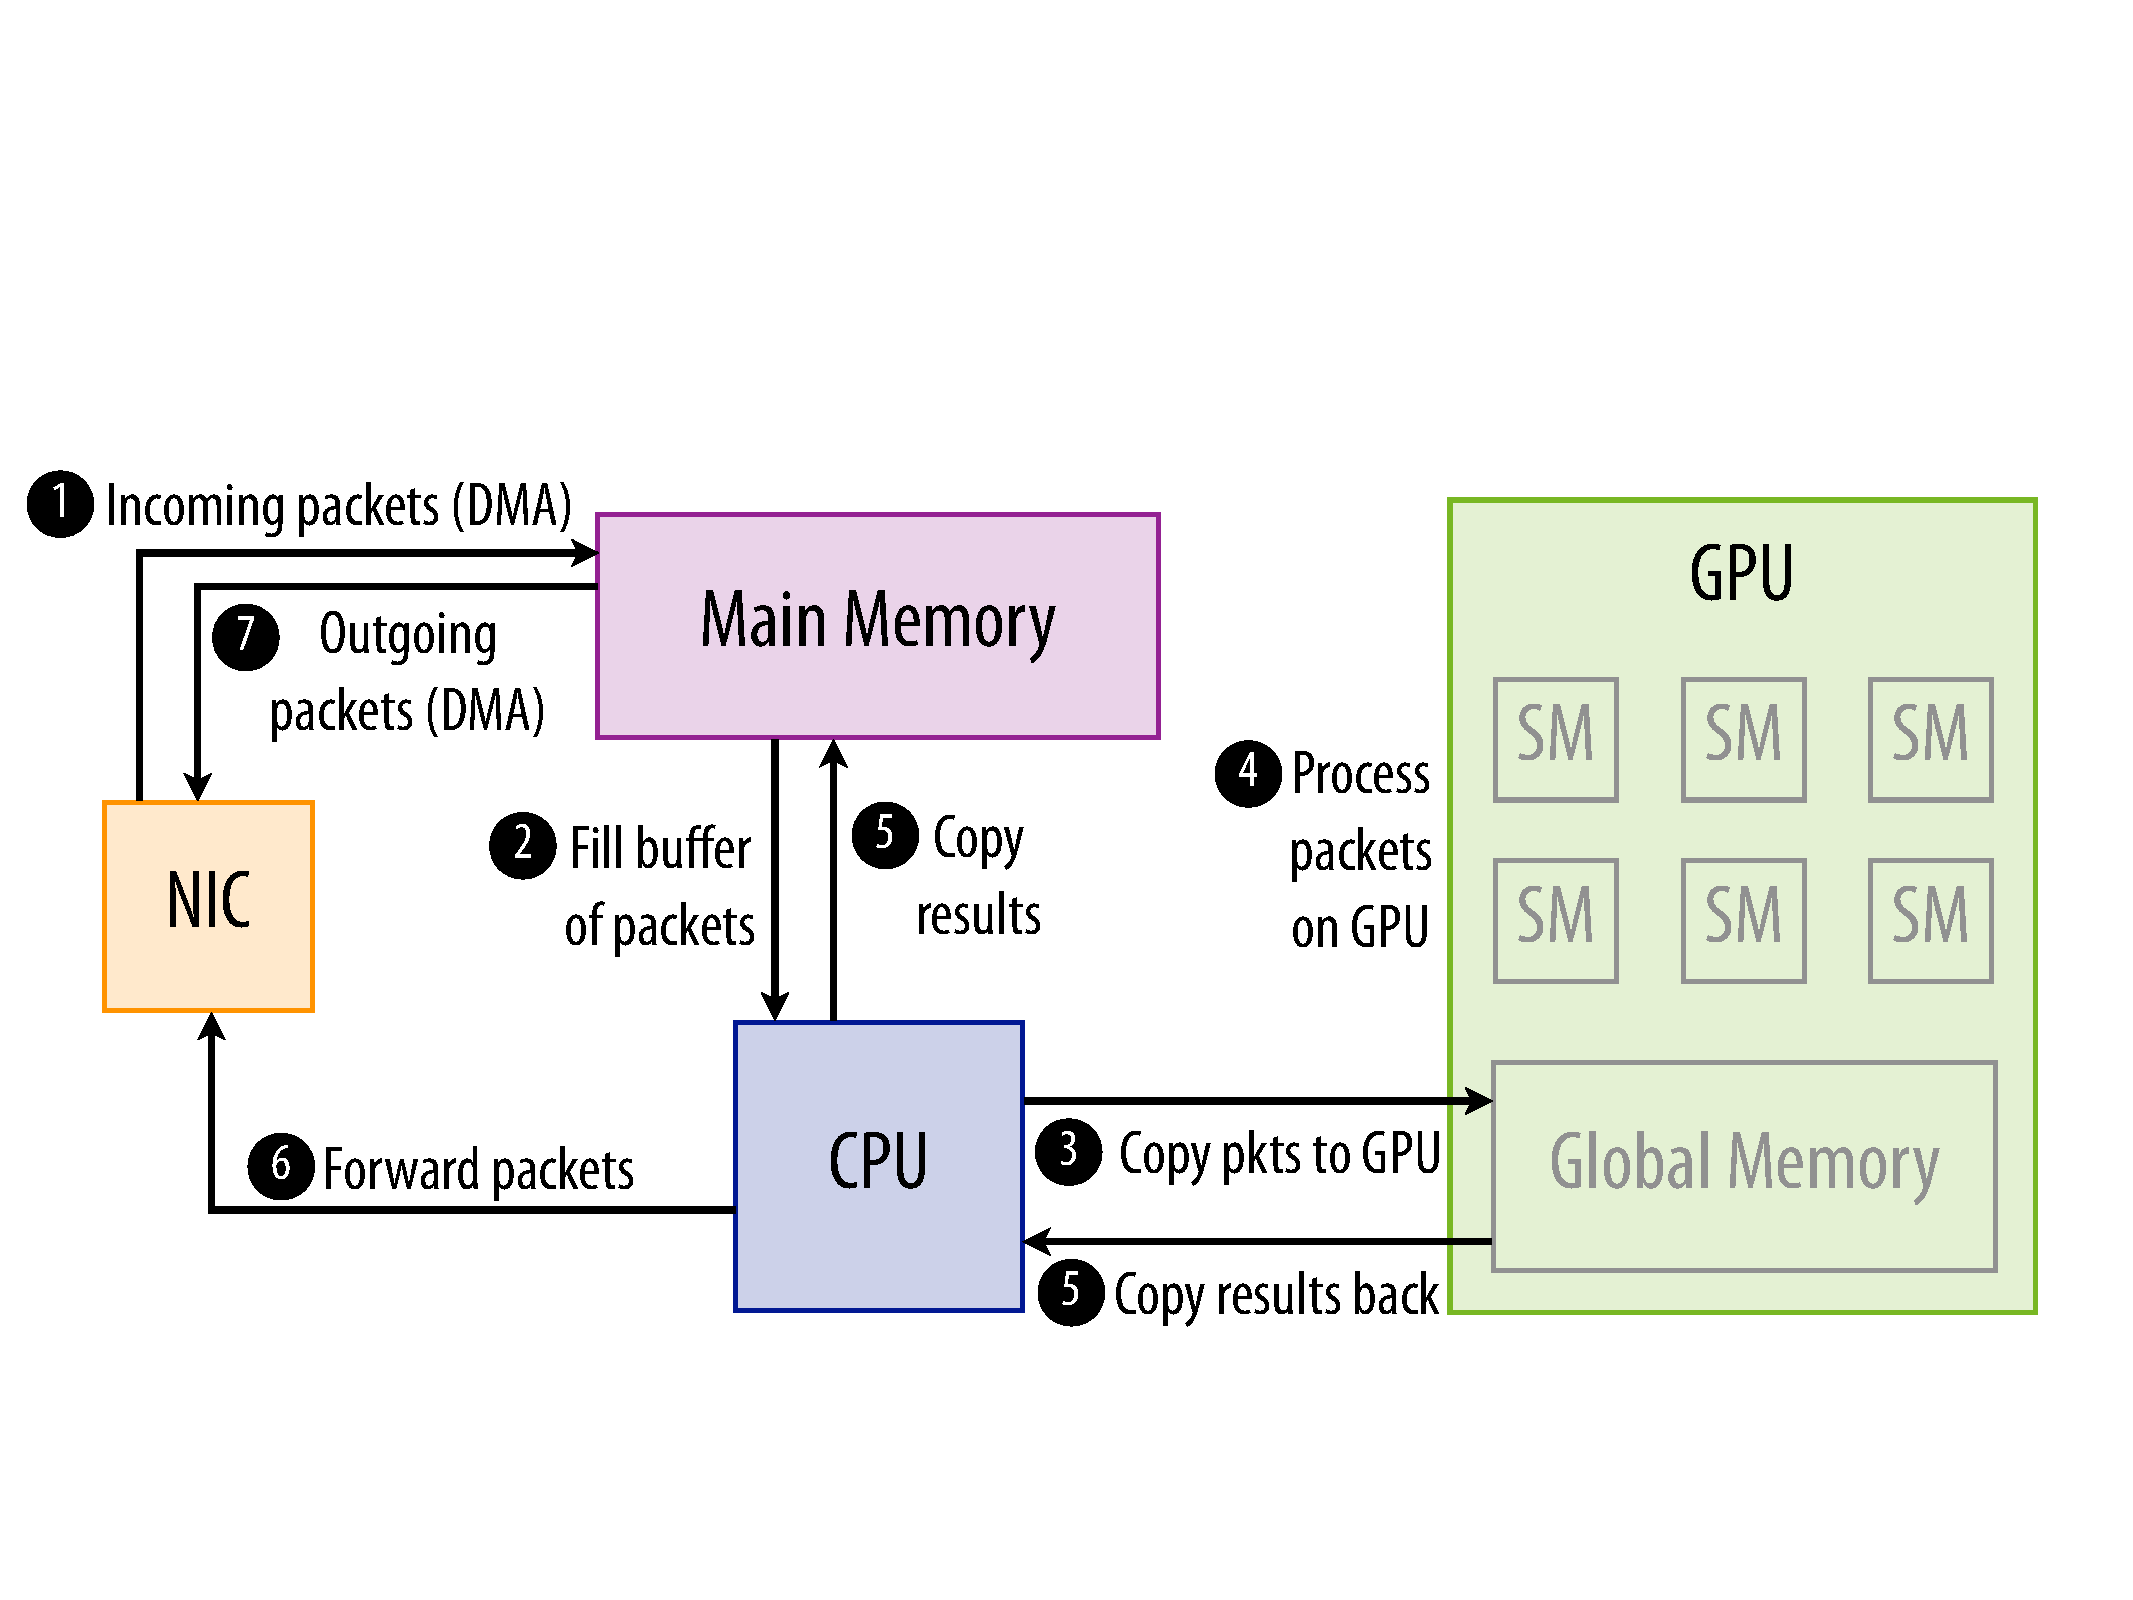
\includegraphics[scale=0.23]{figs/system_overview.pdf} 
   \caption{Basic System Design}
   \label{fig:system}
\end{figure}

\subsection{GPU Programming Issues}
\label{sec:gpu-issues}

\noindent \textbf{Pipelining.} As with almost any CUDA program, ours employs
pipelining for data transfers between main memory and GPU memory. While the GPU
is busy processing a batch of packets, we can utilize the CPU to copy the
results from the previous batch of packets from the GPU back to main memory and
copy the next batch of packets to the GPU (Figure~\ref{fig:pipelining}). In
this way, we never let CPU cycles go idle while the GPU is working.\\

\begin{figure}
   \centering
   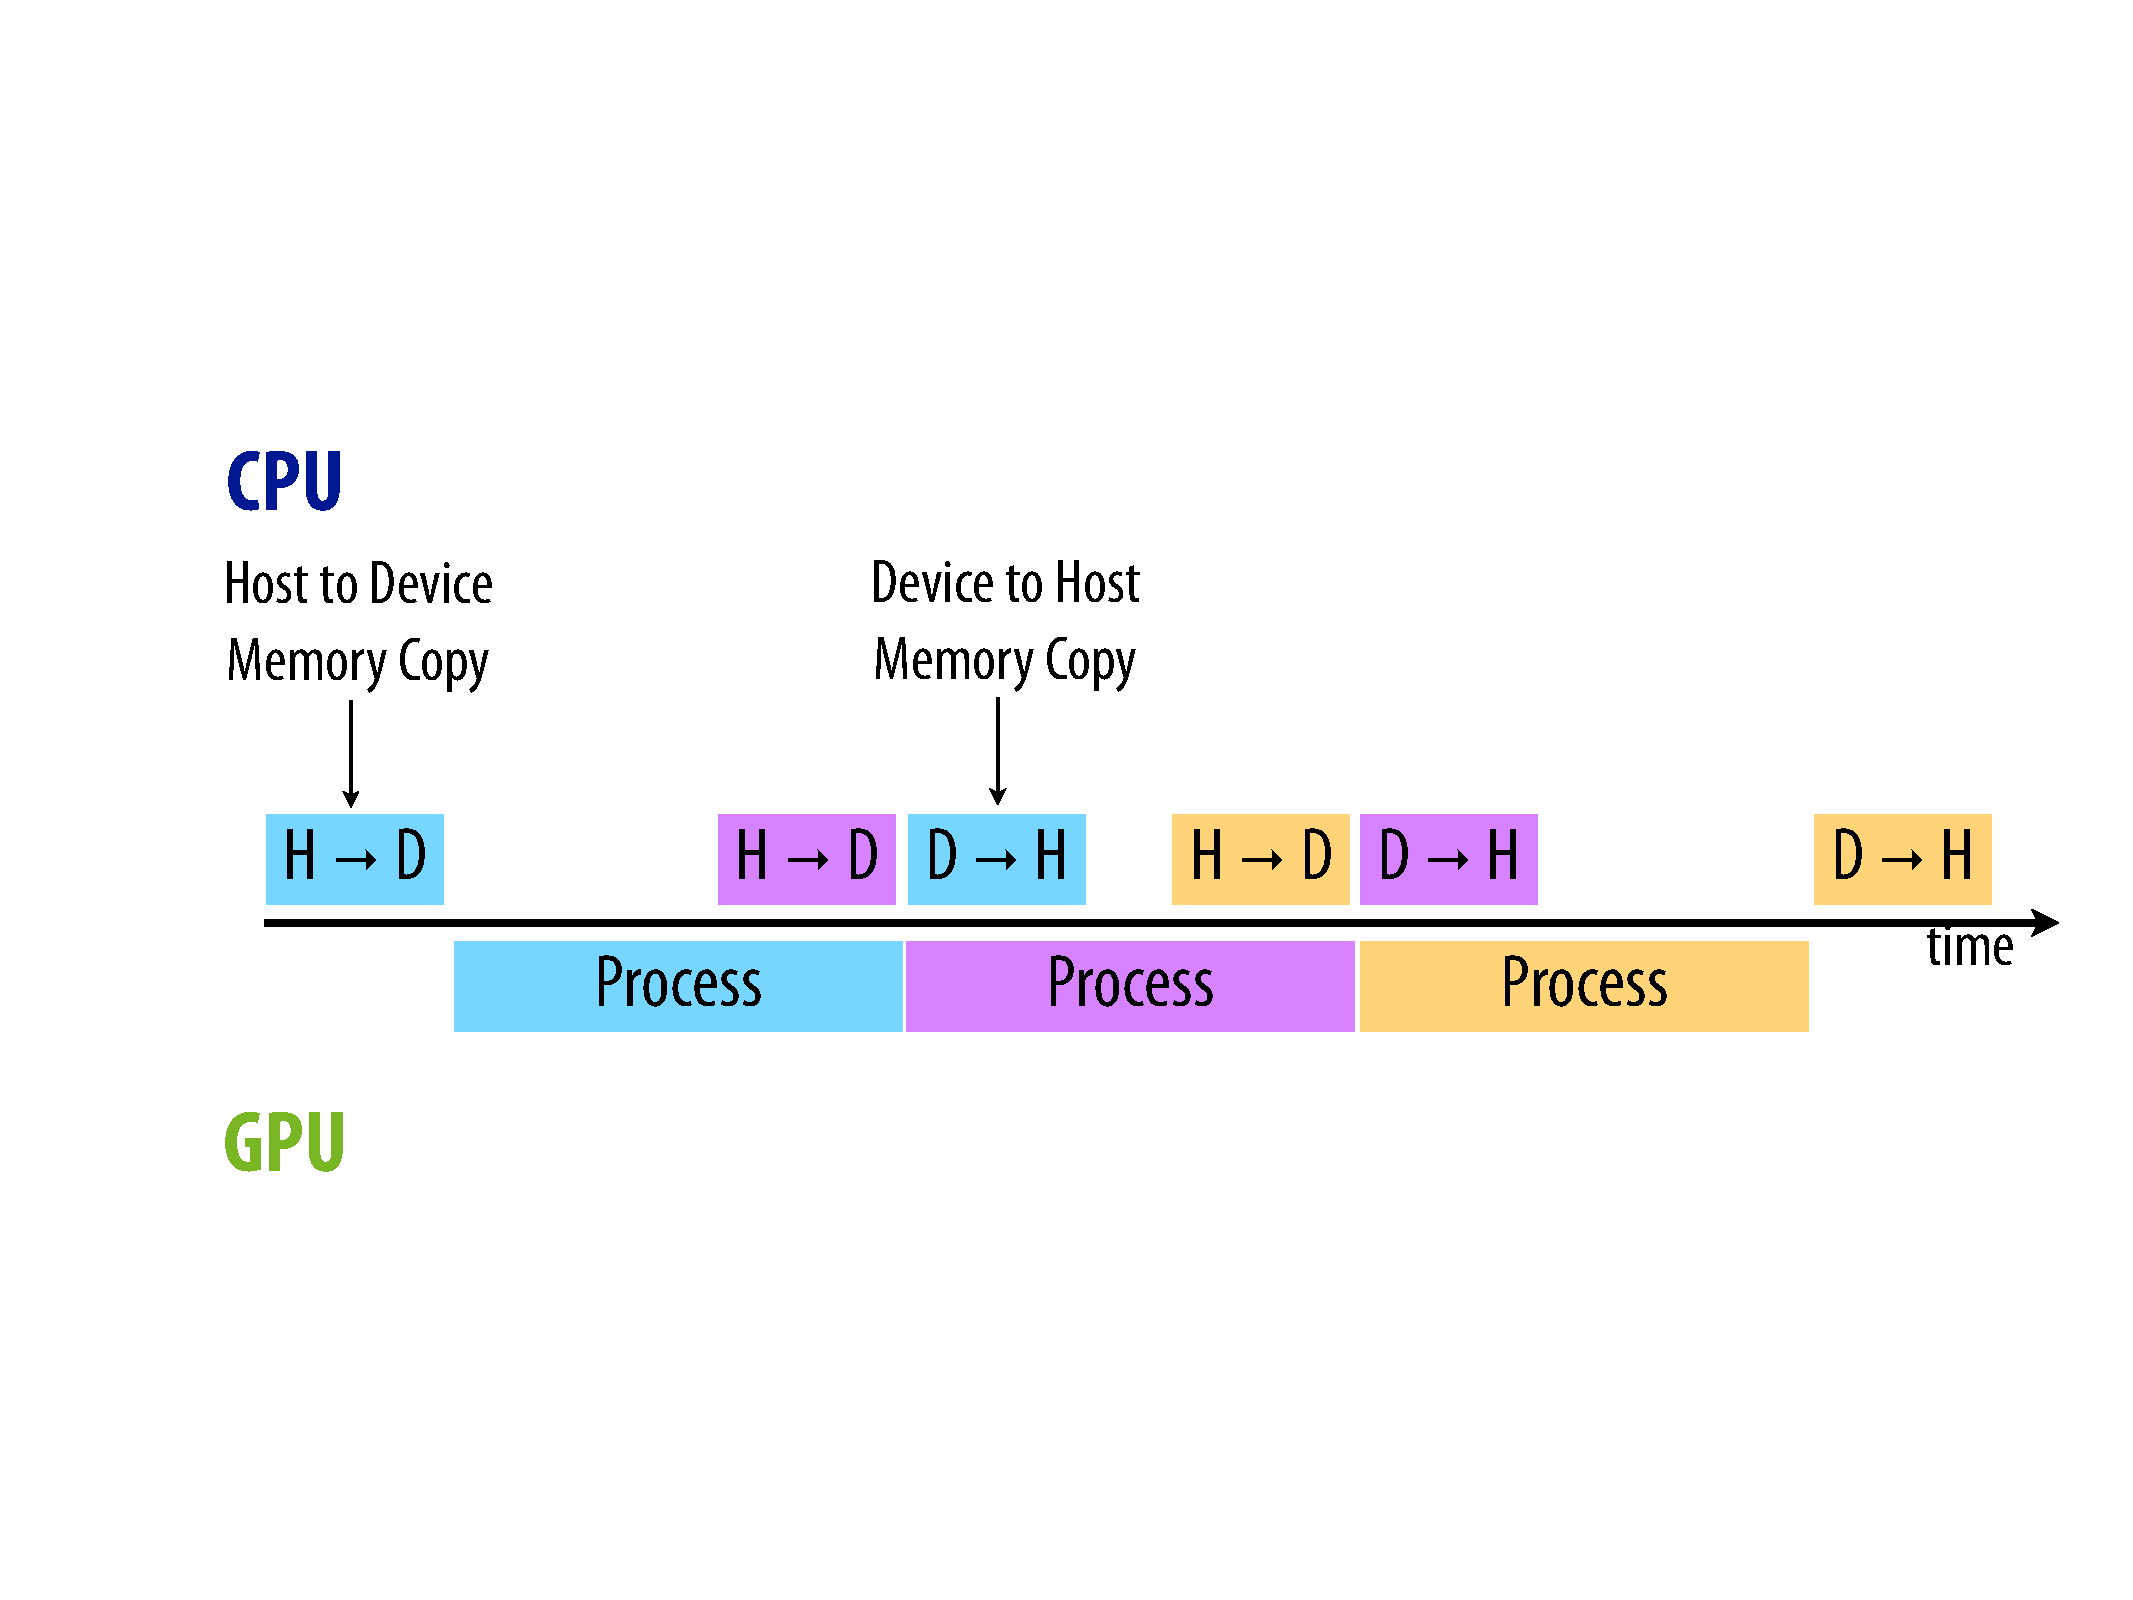
\includegraphics[scale=0.25]{figs/pipelining.pdf}
   \caption{Pipelined Execution}
   \label{fig:pipelining}
\end{figure}

\medskip \noindent \textbf{Batching.} Although the GPU can process hundreds of
packets in parallel (unlike the CPU), there is, of course, a cost: non-trivial
overhead is incurred in transferring packets to the GPU and copying results
back from it. To amortize this cost, we process packets in batches. As packets
arrive at our router, we buffer them until we have a batch of some fixed size
\texttt{BATCH\_SIZE}, at which point we copy the whole batch to the GPU for
processing.

Though batching improves throughput, it can have an adverse effect on latency.
The first packet of a batch arrives at the router and is buffered until the
remaining \texttt{BATCH\_SIZE}-1 packets arrive rather than being processed
right away. To ensure that no packet suffers unbounded latency (i.e., in case
there is a lull in traffic and the batch doesn't fill), we introduce another
parameter: \texttt{MAX\_WAIT}. If a batch doesn't fill after \texttt{MAX\_WAIT}
milliseconds, the partial batch is transferred to GPU for processing. We
evaluate this tradeoff in \S\ref{sec:eval}.

\medskip \noindent \textbf{Mapped Memory.} Newer GPUs (such as ours) have the
ability to directly access host memory that has been \emph{pinned and mapped},
eliminating steps (3) and (5). Though data clearly still needs to be copied to
the GPU and back, using mapped memory rather than explicitly performing the
entire copy at once allows CUDA to copy individual lines ``intelligently'' as
needed, overlapping copies with execution. We evaluate the impact of using
mapped memory in \S\ref{sec:eval} as well.

\subsection{Packet Processing}

A router performs one or more packet processing functions on each packet if
forwards. This includes deciding where to forward the packet (via a longest
prefix match lookup on the destination address or matching against a set of
flow rules) and might also include deciding whether or not to drop the packet
(by comparing the packet header against a set of firewall rules or comparing
the header and payload to a set of intrusion detection system rules).  In our
system we implement two packet processing functions: longest prefix match and
firewall rule matching. \TODO{Justify why?}

\subsubsection{Longest Prefix Match}
\TODO{Bruno: describe trie-based algo and DIR-24-8-BASIC}

\subsubsection{Firewall Rule Matching}

A firewall rule is defined by a set of five values (the ``5-tuple''): source
and destination IP address, source and destination port number, and protocol.
The protocol identifies who should process the packet after IP (e.g., TCP, UDP,
or ICMP). Since most traffic is either TCP or UDP \TODO{cite?}, the source and
destination port numbers are also part of the 5-tuple even though they are not
part of the network-layer header. If the protocol is ICMP, these fields can
instead be used to encode the ICMP message typce and code.

Each rule is also associated with an action (usually ACCEPT or REJECT). If a
packet matches a rule (that is, the values in the packet's 5-tuple matche those
in the rule's 5-tuple), the corresponding action is performed. Rather than
specifying a particular value, a rule might define a range of matching values
for one of the fields of its 5-tuple. A rule might also use a wildcard (*) for
one of the values if that field should not be considered when deciding if a
packet matches. For example, a corporate firewall might include the following
rule: (*, [webserver-IP], *, 80, TCP):ALLOW. This rule allows incoming traffic
from any IP address or port to access the company's webserver using TCP on port
80.

Our rule matching algorithm is incredibly simple. Rules are stored in order of
priority and a packet is checked against each one after the next in a linear
search. Though this sounds like a na\"{i}ve approach, \cite{Rovniagin} claims
that it is the approach taken by open source firewalls like \texttt{pf} and
\texttt{iptables} and likely other commercial firewalls as well. We discuss how
we generate the rules used in our tests in \S\ref{sec:eval-proc}.

\section{Evaluation}

\subsection{Experimental Setup}

\subsubsection{Hardware}

\subsubsection{Packet Generation}

\subsubsection{Packet Processing}

\noindent \textbf{Longest Prefix Match.} Describe the FIB we use...\\

\noindent \textbf{Firewall Rule Matching.} Describe our rules...


\subsection{Evaluation Metrics}

\noindent \textbf{Bandwidth.} \\

\noindent \textbf{Latency.} \\

\noindent \textbf{Processing Time.}


\subsection{Results}

\section{Discussion and Future Work}
\label{sec:disc}

\noindent \textbf{Multithreaded CPU Processing.} The comparison of our CPU/GPU
router to the CPU-only baseline is not completely fair. Our CPU-only router
operates in a single thread, yielding misleadingly low performance. Any
CPU-based software router in the real world would certainly spread packet
processing across multiple cores, and we would be surprised if any core
software router were run on a machine with fewer than 16 cores.

A simple extension of our project would be to parallelize our CPU-only packet
processing functions with OpenMP to provide more realistic baseline
measurements.

\medskip \noindent \textbf{Harder Processing Functions.} Even in the final
iteration of our router, the CPU/GPU version only achieves slightly more than
three times the bandwidth of the CPU-only version. Though this is by no means
an improvement to scoff at, the speedup strikes us as being a tad low. We
suspect the cause is that our packet processing functions are not taxing
enough; the harder the processing function, the more benefit we should see from
the massively parallel GPU. This suggests that GPU-based software routers might
be best suited for complex packet processing like IDS filtering (which requires
pattern matching against packet payloads) and IPsec processing (which requires
expensive cryptographic operations).

One of our goals was to explore the best way to schedule multiple packet
processing functions on the GPU. As a simple example, to schedule both LPM and
firewall lookup, you could imagine parallelizing per-packet or prallelizing
per-function (Figure~\ref{fig:scheduling}). We began testing these schemes,
but, as our processing functions turned out to be ``easy,'' there was little
difference. We think this is still an interesting question to explore with more
taxing processing functions.

\begin{figure}
    \centering
    \subfigure[Per-packet]{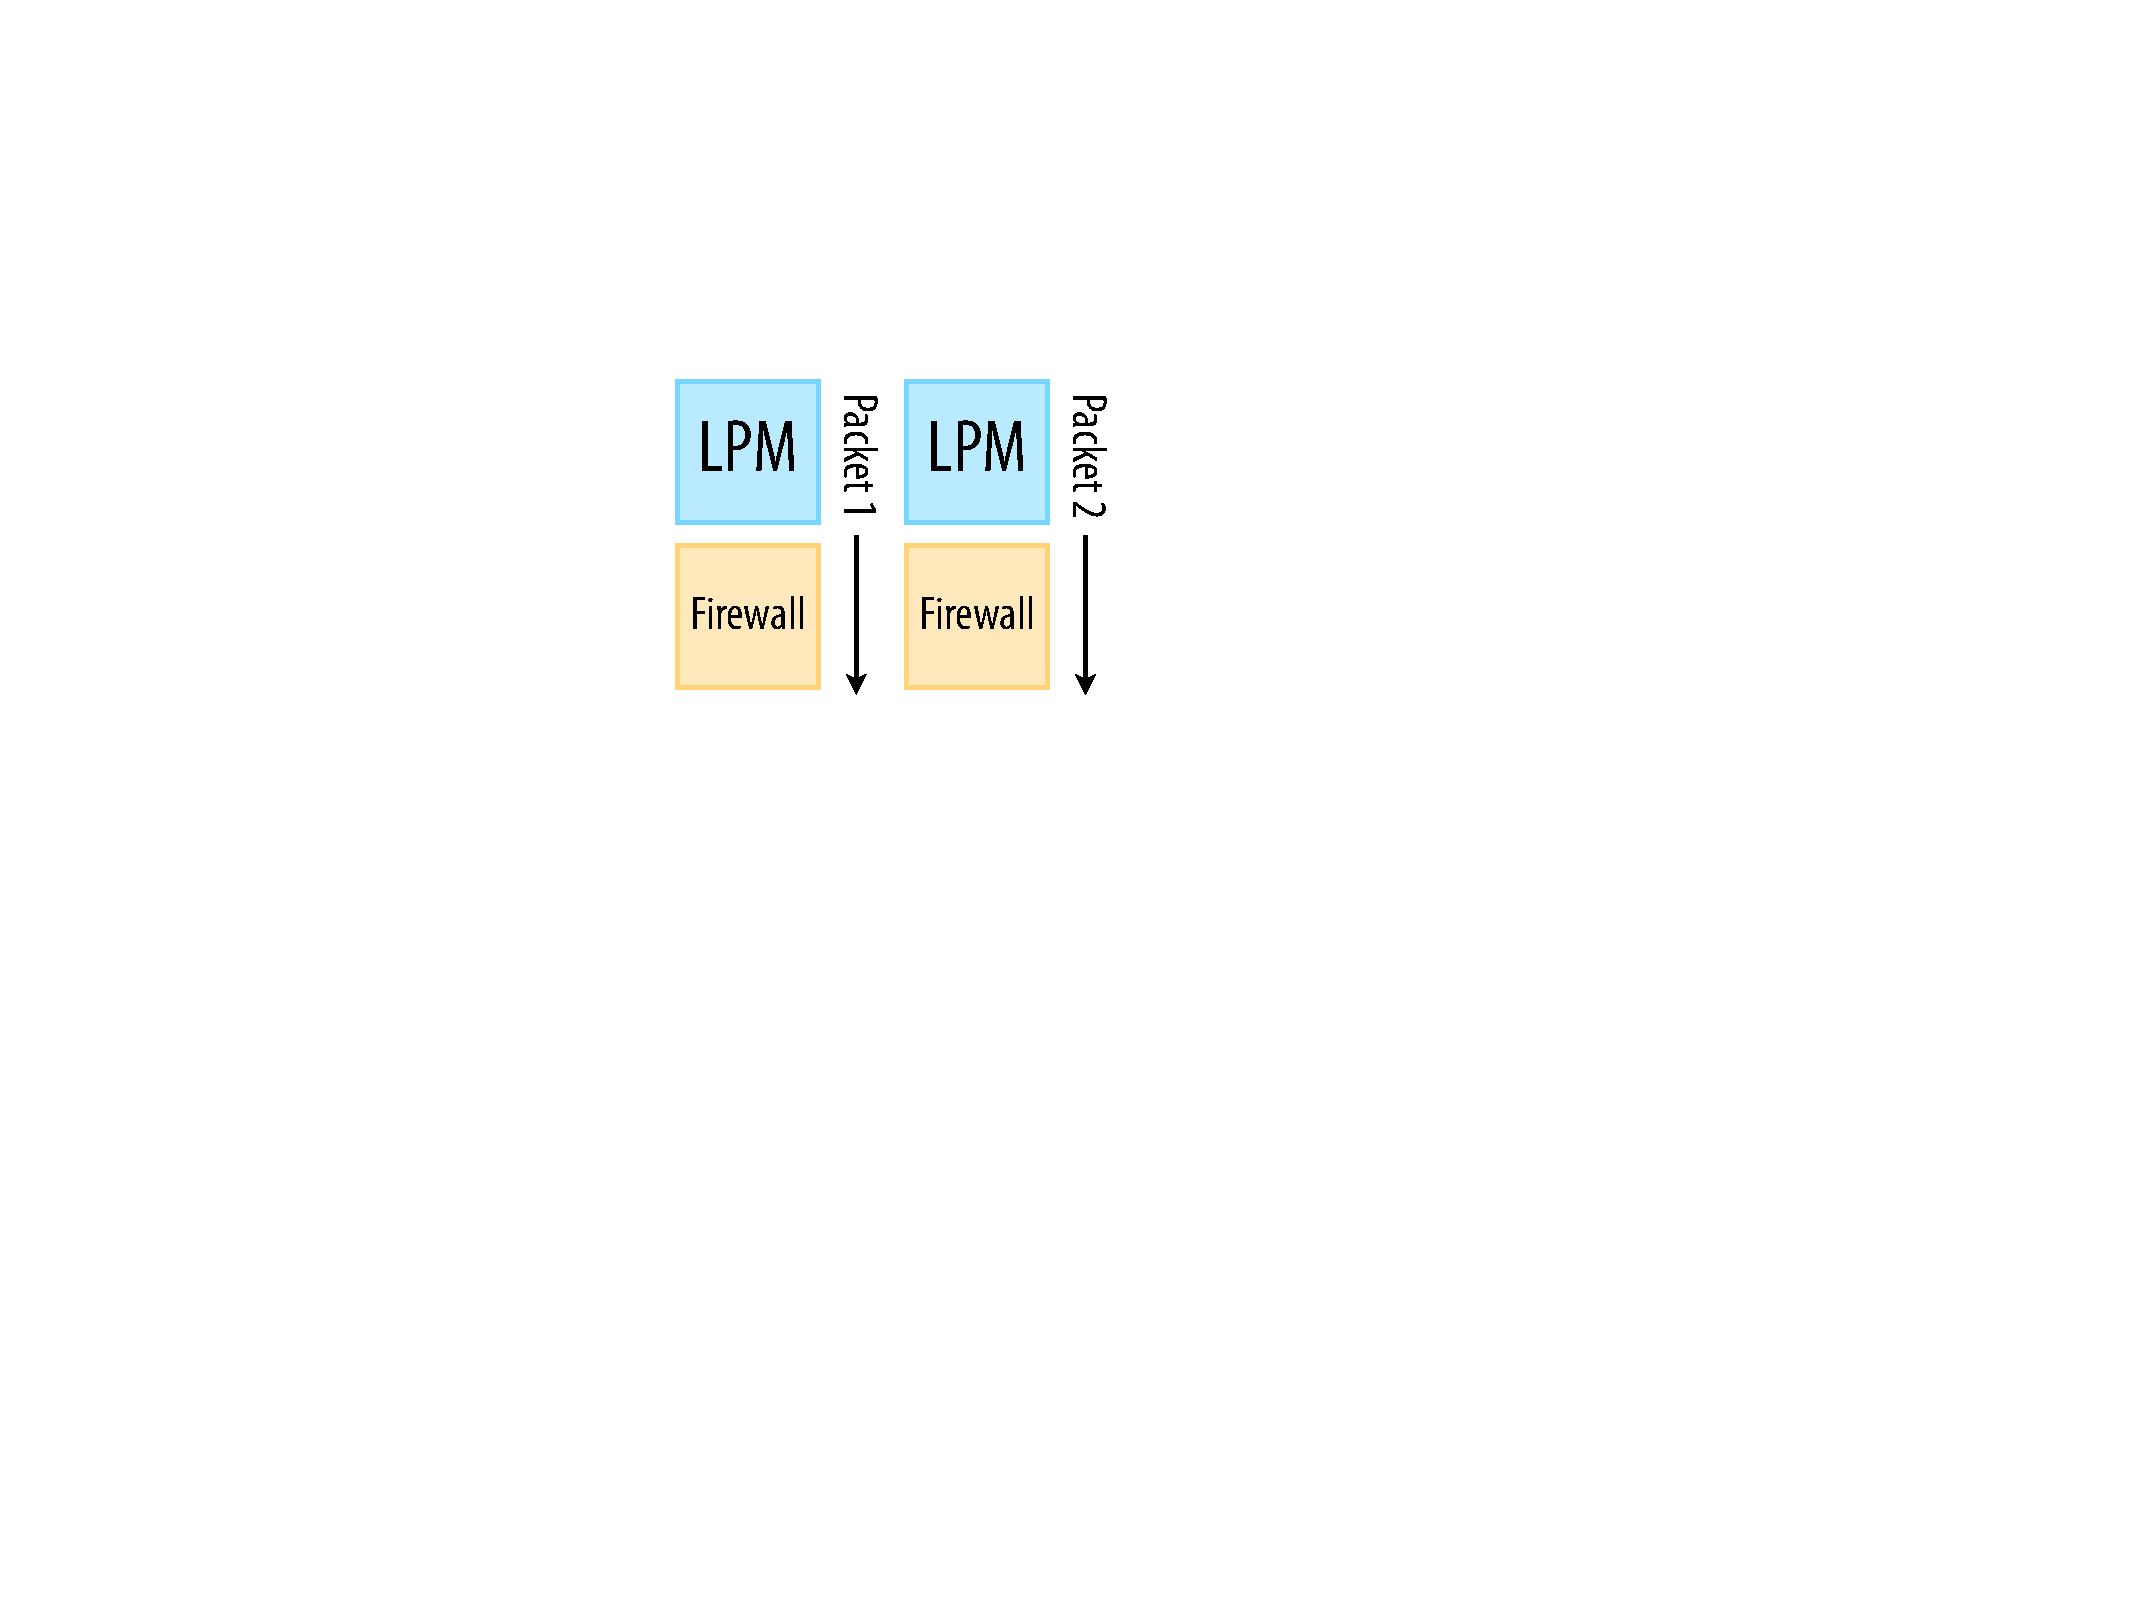
\includegraphics[height=3cm]{figs/per-packet-par.pdf}\label{fig:per-packet-par}}

	\medskip
    \subfigure[Per-function per-packet]{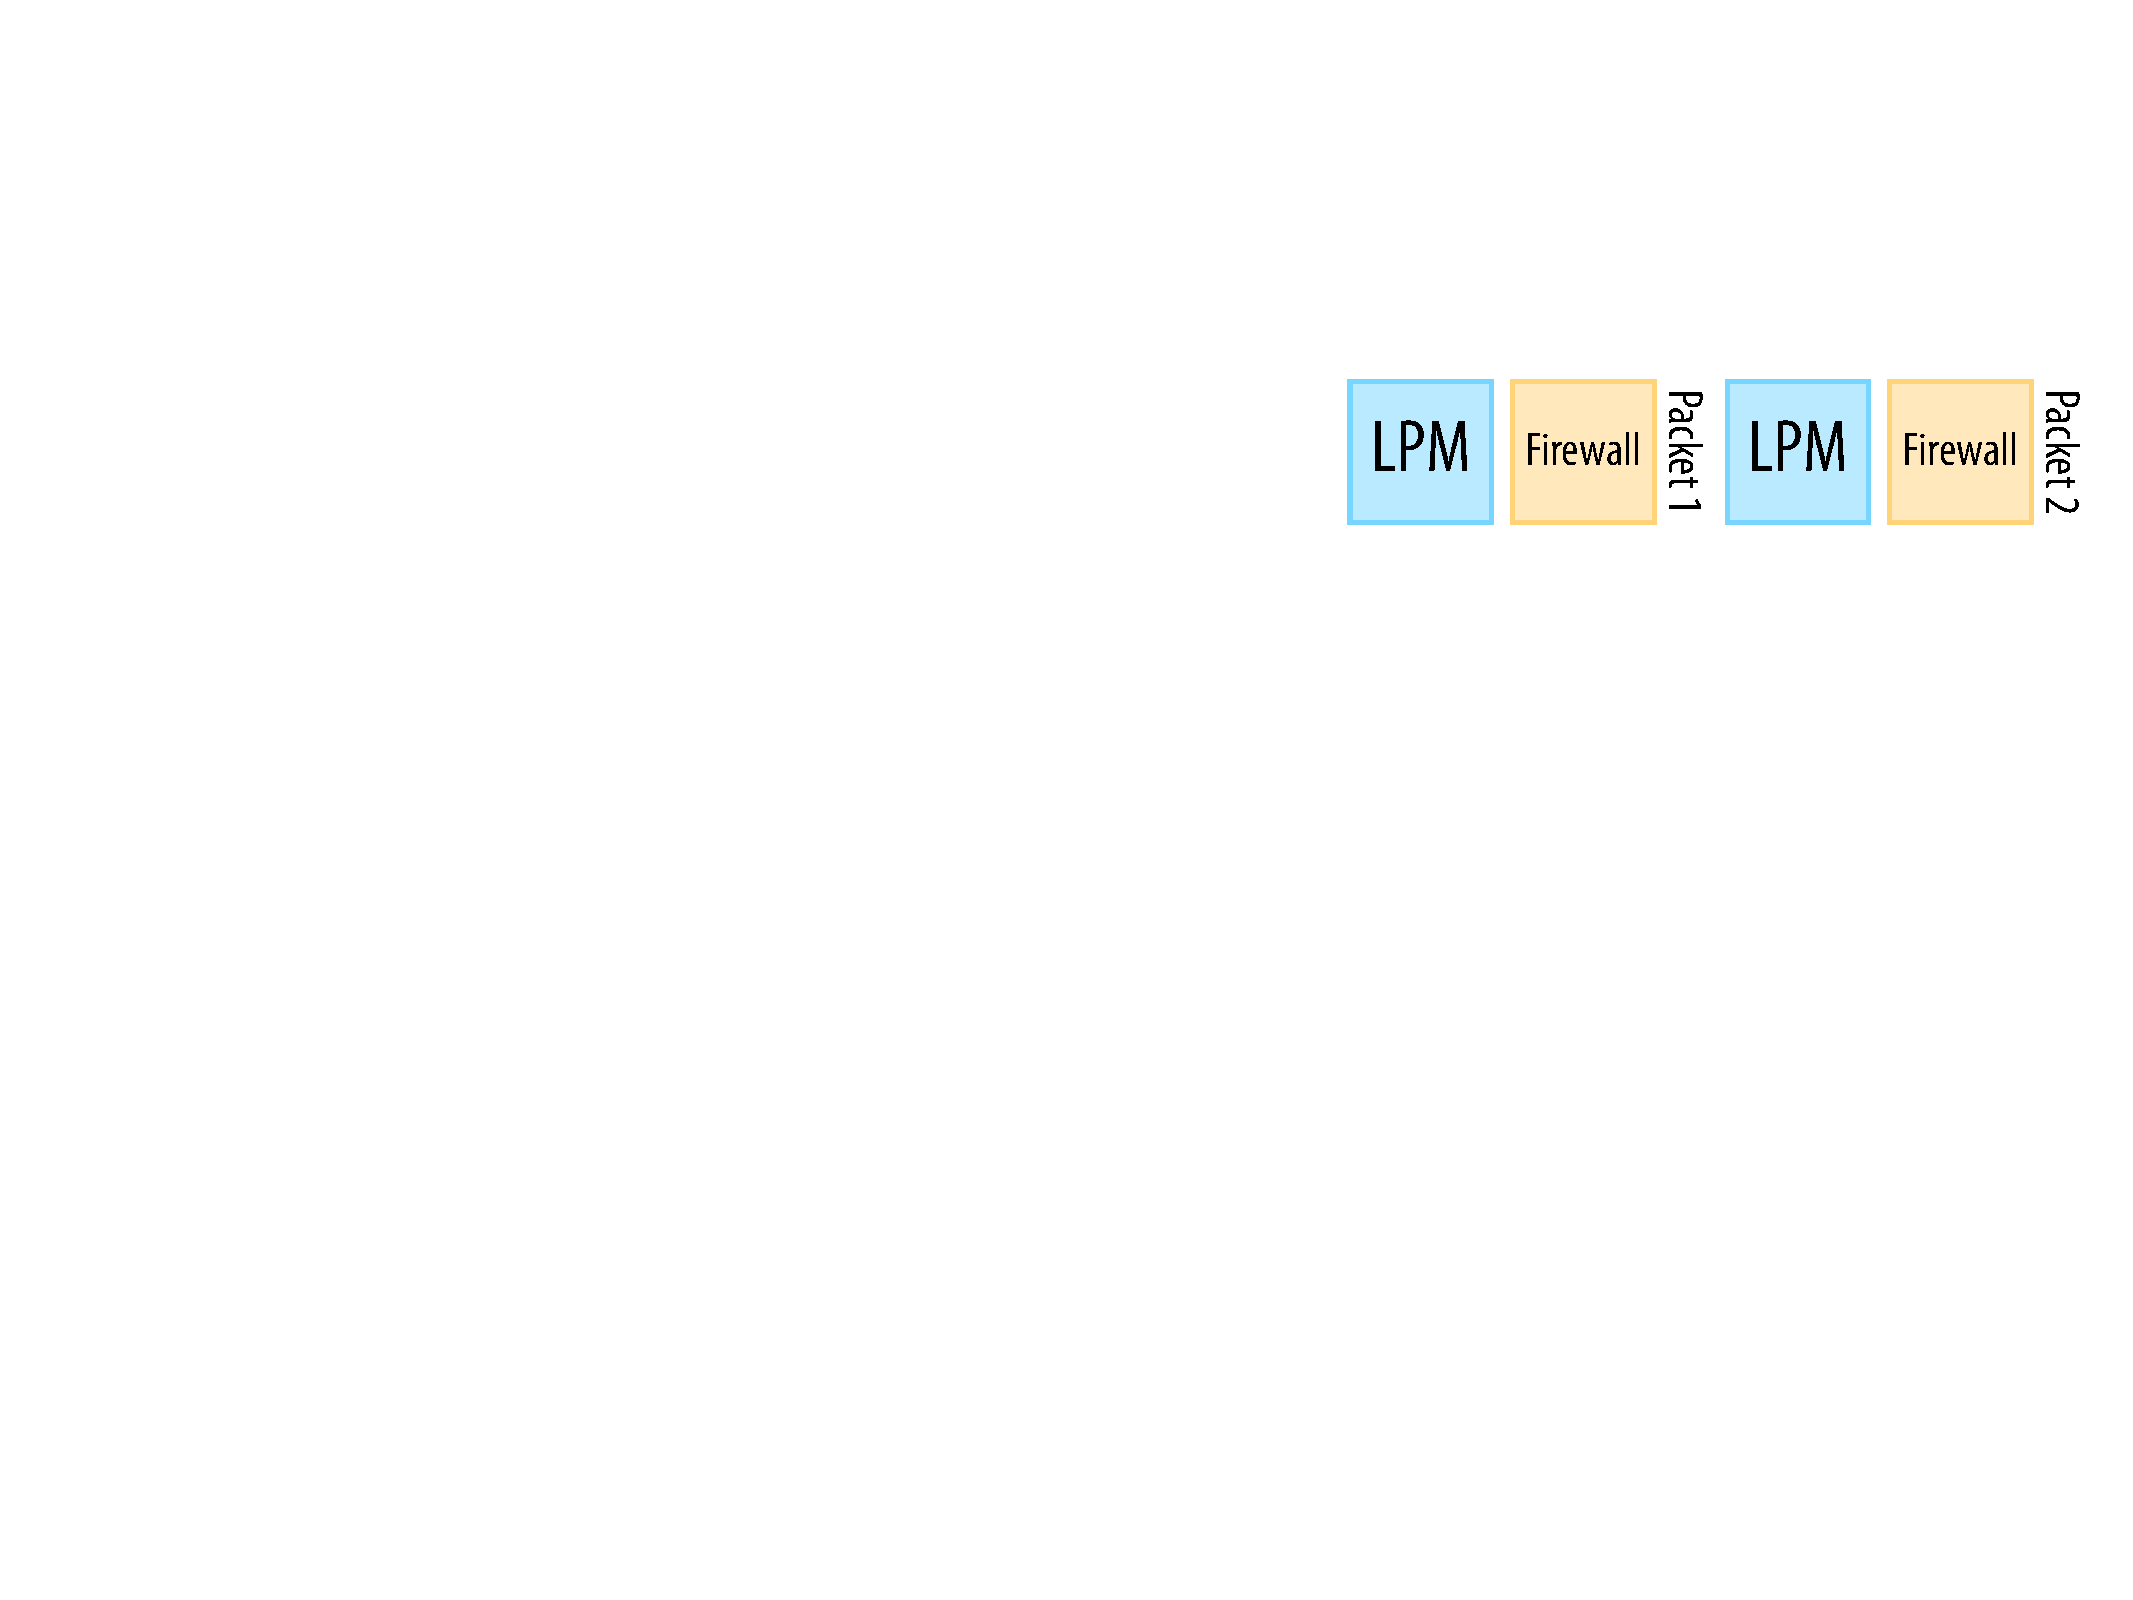
\includegraphics[height=1.5cm]{figs/per-function-par.pdf}\label{fig:per-function-par}}

    \caption{Scheduling Multiple Processing Functions}
	\label{fig:scheduling}
\end{figure}

\medskip \noindent \textbf{Faster Packet I/O.} By far the largest issue we noted
is that generating and gathering packets from Click contributes to the majority
of the latency, becoming the dominant part of both CPU and GPU overall
latency. As seen in Figure \ref{fig:iter4}, removing the overhead contributed by
generating and gather packets, our GPU implementation performs much better than
our CPU implementation. This is the same conclusion that the authors of
PacketShader \cite{Han} came to. Thus in their system, they focused on
reimplementing the driver for their NIC to alleviate these issues. In our
framework we could similarly emulate newer NIC technologies (like RDAM) to allow
zero-copy access to DRAM that is memory mapped in the GPU. We could emulate this
by having Click copy packets directly to application DRAM rather than first
sending the packets to the application via a socket.

\medskip \noindent \textbf{Streams.} The typical use of a GPU involves the
following operations: a set of tasks and input data is first collected,
transferred to the GPU, processed, and eventually the output is copied back to
the host device. These operations are performed cyclically, often on
independent data, as in the case of our packet processing applications. Since
the CUDA and host device are separate processing unit, it is critical for
performance to maximize the concurrency of such operations.

CUDA Streams provide an interesting mechanism to optimize GPU-based
applications. Basically, CUDA allows to assign operations (like kernel
execution and \emph{asynchronous} data transfer to and from the device) to
streams. Then, the stream executions are overlapped in such a way that similar
operations of different stream do not interfere with each other (i.e., a kernel
execution in stream1 and a data transfer in stream2 can be performed in
parallel). The high level idea is quite similar to that of instruction
pipelining.

We have implemented a version of our router using CUDA streams. Our preliminary
results show that streams indeed increase the parallelism and throughput.
Operation overlapping is quite visible in the Visual Profiler. The number of
processed packets increases substantially (around 30-40\%). However, more
investigation is required on this subject, particularly on the packet generator
and on the new issues related to resource management, highlighted by the Visual
Profiler.

%\TODO{Bruno: Briefly describe CUDA's built-in streams funcitonality}

\medskip \noindent \textbf{Integrated Graphics Processors.} One tempting idea
to explore is the use of integrated graphics processors rather than dedicated
discrete GPUs. Modern processors (Intel Core i-series, etc.) include a
traditional multi-core GPU directly on the processor itself. In essence, this
shifts the position of the GPU from being on the PCI-express bus to being
co-located with the CPU on the quickpath interconnect (QPI). As the QPI can
potentially provide more bus bandwidth to memory, and integrated graphics
processor could obtain even higher maximum throughput, as memory constraints
are the biggest source of potential slowdown after packet I/O at the NIC.

\section{Conclusion}

\TODO{general conclusion stuff}



\newpage
{\small
\bibliographystyle{abbrv}
\bibliography{refs}
}

\appendix
\section{Distribution of Credit}
\begin{center}
   \begin{tabular}{ l l } 
      \toprule
      \textbf{Group Member}  & \textbf{Portion of Credit} \\
      \midrule
	  Matt & 33.3\% \\
      David & 33.4\% \\
	  Bruno & 33.3\% \\
      \bottomrule
   \end{tabular}
\end{center}


\end{document}
